\subsection{Cross Sections as a function of the proton momentum}
%Results in P$_{p}$ }

The differential cross section in terms of P$_{p}$ for interactions on the various nuclear targets are shown in Fig.~\ref{figure:xsec_proton_p}. P$_{p}$ is the magnitude of the proton momentum in GeV/c.  This might be sensitive to nuclear effects since the proton passes through some nuclear matter before emerging.  The uncertainties broken down by source for both the absolute cross sections and the cross section ratios as a function of P$_p$ can be found in Fig.~\ref{fig:xsec_err_proton_p}.

% tki_proton_p xsecs
\begin{figure}[h] 
	\centering
  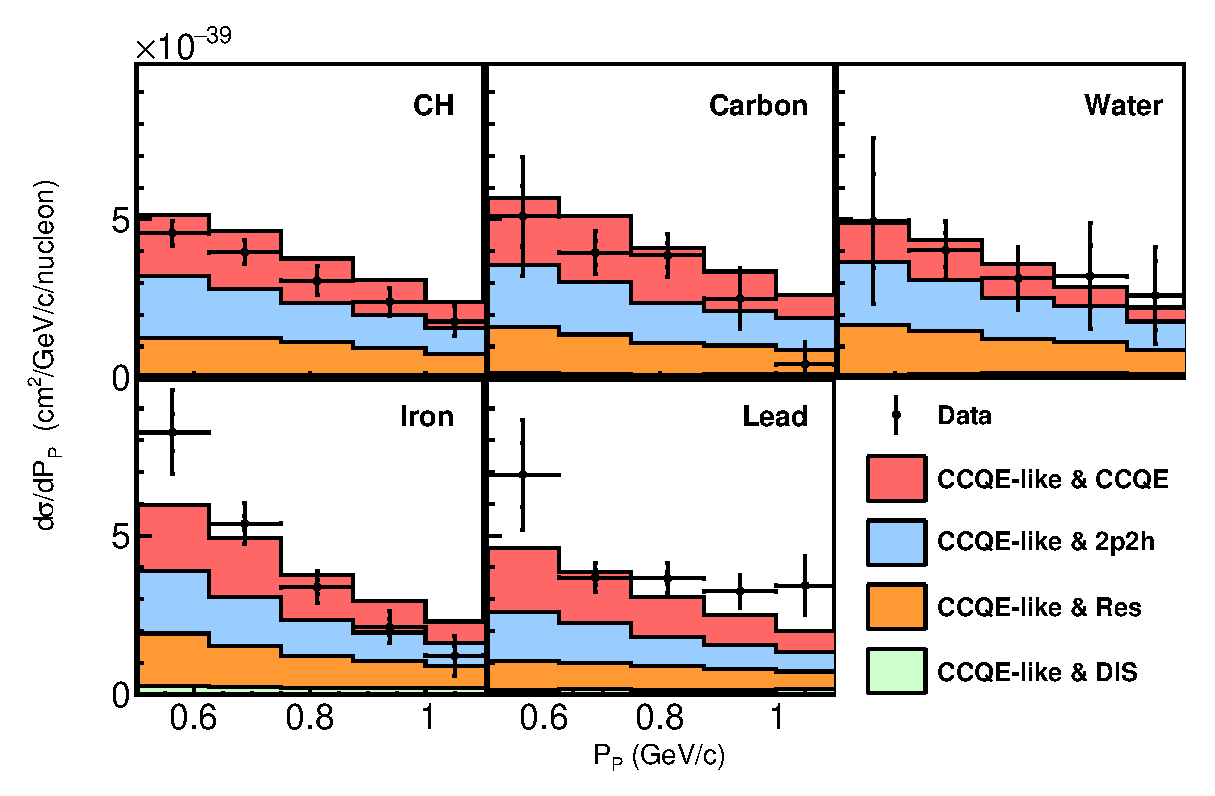
\includegraphics[width=\linewidth]{Figures/xsec_five_square/proton_p.eps}
	\caption{The differential cross section as a function of P$_p$ for CH, C, H$_{2}$O, Fe, and Pb targets, along with the predictions for the different quasielastic-like signal processes.}
	\label{figure:xsec_proton_p}
\end{figure}

The MINERvA tune simulation models the data fairly well for each target except Fe and Pb.  For the Fe target, there is an indication of a shape difference, where the data has a slightly softer momentum distribution.  This is different from what is seen in Pb where there is a markedly harder distribution at high momentum than the model.

The differential cross sections in P$_{p}$ for the different targets are compared to a range of models in Fig.~\ref{fig:models_proton_p}. NEUT exhibits a higher cross section than the data, in general, with a shape that agrees with the data for the smaller targets.  For the Pb target, NEUT and the hN GENIE models have a considerably softer momentum shape than the data, indicating too much FSI as seen in the other variables.  The other models do a fairly good job describing the data.
The \chisq\ between the cross sections and the models can be found in Table~\ref{tab:protonmomentum}.

% comparisons to generators proton_p
\begin{figure}
    \centering
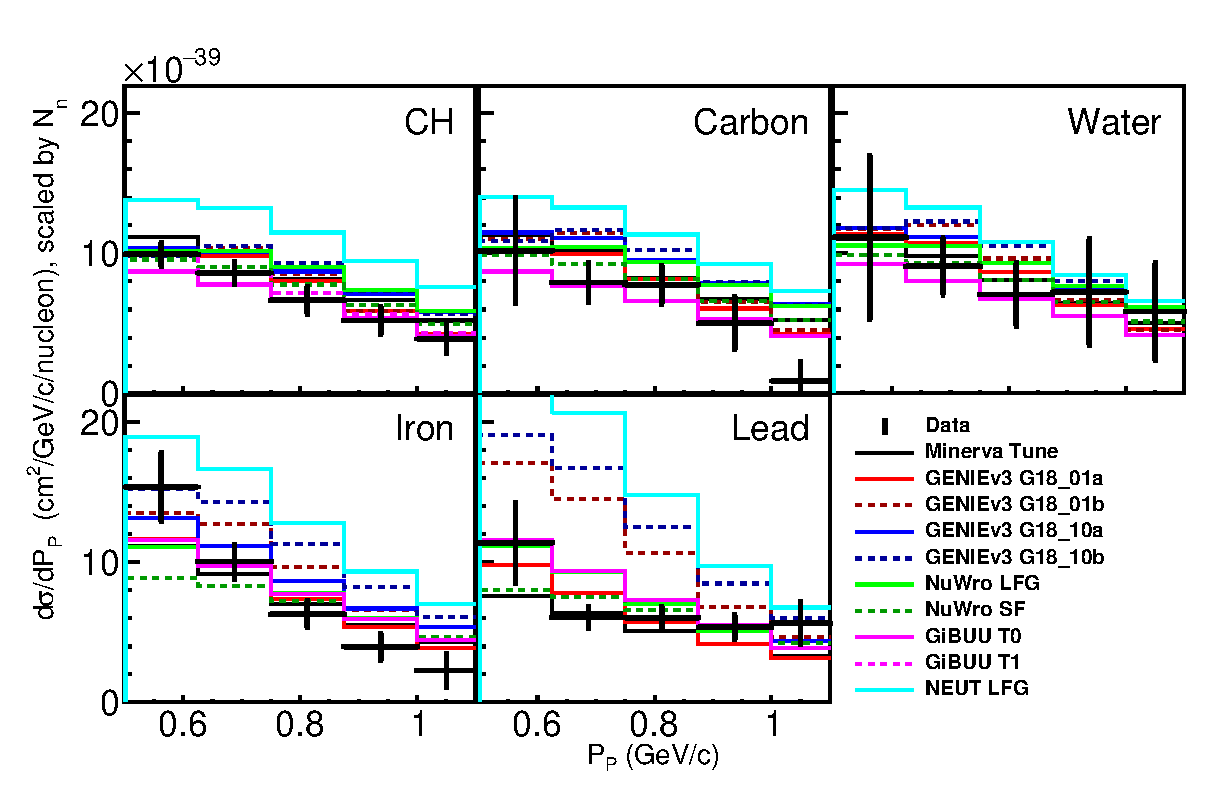
\includegraphics[width=\linewidth]{Figures/gencompare/proton_p_5square.eps}
    \caption{Cross section measurements and predictions as a function of P$_p$ for different targets and for a selection of different generator and model choices.}
    \label{fig:models_proton_p}
\end{figure}

The ratio of the differential cross section for each target relative to that for scintillator as a function of  P$_{p}$  is shown in 
Fig.~\ref{Figure:Gencompare_proton_p_ratio}. The ratio is higher for NEUT than the data for all of the targets and the other models.  For the Pb target the hN versions of GENIE approach NEUT and exhibit a higher ratio at low momentum that the data, as does NEUT.  This may indicate that the FSI strength for NEUT and the hN versions of GENIE becomes excessive for Pb as compared to what happens for the smaller targets.
The \chisq\ between the cross section ratios and the models can be found in Table~\ref{tab:protonmomentum}.

\begin{figure}
    \centering
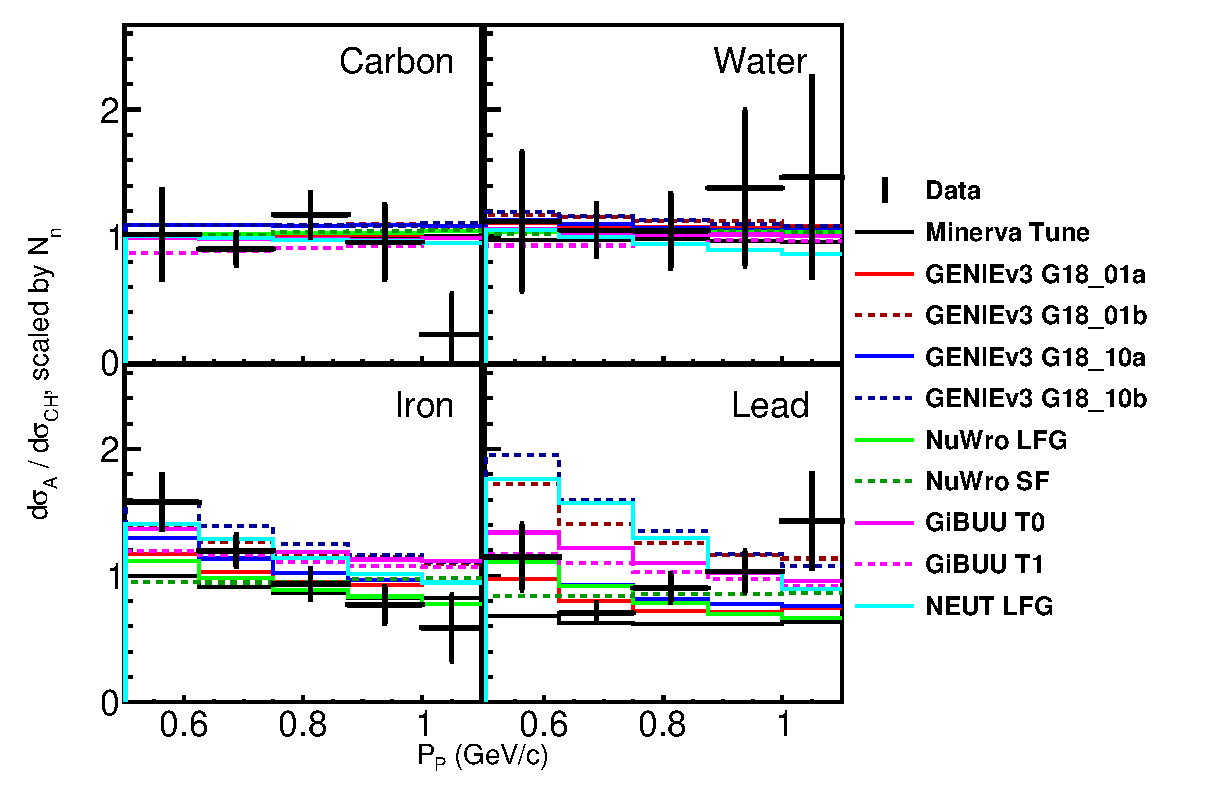
\includegraphics[width=\linewidth]{Figures/gencompare/proton_p_4square.eps}
    \caption{P$_{p}$ cross-section ratio generator comparison for multiple targets.  Changes to the FSI model (GENIE ``a'' to ``b'') in GENIE change the cross section ratio most at low proton momenta, and those changes are larger than changes to the 2p2h model (GiBUU T0 to GiBUU T1) or changes to the initial state (GENIE 1 to GENIE 10) or (NuWro LFG to NuWro SF).}
        \label{Figure:Gencompare_proton_p_ratio}
\end{figure}
